\documentclass{beamer}
\usepackage[utf8]{inputenc} 
\usepackage[french]{babel}
\usepackage[T1]{fontenc}
\usetheme{default}
\usecolortheme{beaver}
\usepackage{graphicx} %affichage des images  
\usepackage{hyperref} %pour les liens
\usepackage{multicol} %pour bien afficher les références
\usepackage{listings} %pour afficher des lignes de code
\usepackage{multimedia}
\usetheme{CambridgeUS}
\setbeamertemplate{footline}[frame number] %numerotation des pages

\title{\textbf{Tables arc-en-ciel}}
\author{FAUQUETTE Mael, MAHIER Awen, RABOT Valentin, TRANSON Alexandre}
\institute{L3 Informatique Groupe 3A}
\date{4 avril 2024}

\begin{document}

\begin{frame}
\titlepage
\centering
\includegraphics[scale=0.3]{img/LogoUniCaen.png}
\end{frame}

\begin{frame}
\frametitle{Sommaire}
\tableofcontents
\end{frame}

\section{Introduction}
\begin{frame}
\frametitle{Introduction}
\framesubtitle {Description du projet}
\begin{block}{Tables arc-en-ciel}
$\Rightarrow$ Structure de données qui réduit les temps de calcul pour retrouver un mot de passe au prix d'un coût en espace.\newline 
$\Rightarrow$ Stockent des hashs afin de vérifier facilement si une empreinte existe et son mot de passe correspondant.
\end{block}
\end{frame}

\begin{frame}
\frametitle{Introduction}
\framesubtitle {Tables arc-en-ciel}
\begin{center}
\end{center}
\begin{figure}[H]
\centering
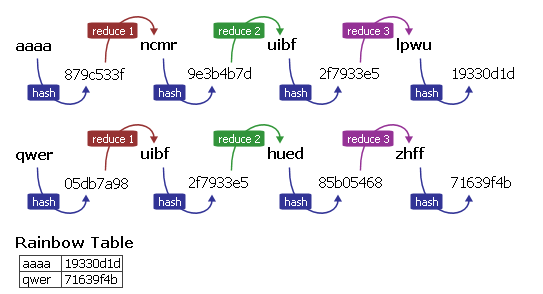
\includegraphics[height=5.5cm]{img/fonctionnement.png}
\caption{Génération d’une rainbow table}
\end{figure}
\end{frame}

\section{Problématique}
\begin{frame}
\frametitle{Problématique}
\framesubtitle {Description de la problématique }
\begin{center}
    \textbf{Comment créer une table arc-en-ciel fonctionnelle et optimisée ?}
\end{center}
\begin{block}{Principaux objectifs :}
\begin{itemize}
\item Générer une base synthétique de mots de passe hachés.
\item Implémenter une table arc-en-ciel paramétrable.
\item Implémenter des optimisations de la table arc-en-ciel.
\item Étude comparative des performances en fonction des paramètres.
\end{itemize} 
\end{block}
\end{frame}

\section{Décomposition des tâches}

\begin{frame}
\frametitle{Décomposition des tâches}
\framesubtitle {Répartition du travail}
\begin{block}{}
\begin{itemize}
    \item Génération des mots de passe et stockage de leurs hash : Awen
    \item Fonction de réduction et comparaison des hash : Mael
    \item Rapport, diaporama et récupération des données : Valentin
    \item Interface graphique et hachage des mots de passe : Alexandre
\end{itemize}
\end{block}
\end{frame}

\section{Fonctionnalités}

\begin{frame}
\frametitle{Fonctionnalités}
\framesubtitle {Génération des mots de passe}
\begin{block}{}
$\Rightarrow$ Parcours d'un hash.\newline
$\Rightarrow$ Calcul d'une graine qui sera utilisée avec la classe Random.\newline
$\Rightarrow$ Une longueur pour le mot de passe entre 8 et 32 caractères.
\end{block}
\end{frame}

\begin{frame}
\frametitle{Fonctionnalités}
\framesubtitle {Dé-hachage d'un mot de passe}
\begin{block}{}
Impossible avec un algorithme de hachage sécurisé comme SHA-256. Ce processus est unidirectionnel, il est conçu pour être irréversible.
\end{block}
\end{frame}

\begin{frame}
\frametitle{Fonctionnalités}
\framesubtitle {Stockage des mots de passe}
\begin{block}{}
$\Rightarrow$ Dans un fichier texte.\newline
$\Rightarrow$ Première ligne la profondeur et la liste des couleurs.\newline
$\Rightarrow$ Chaque ligne représente un mot de passe d'origine et un hash.
\end{block}
\begin{figure}[H]
\centering
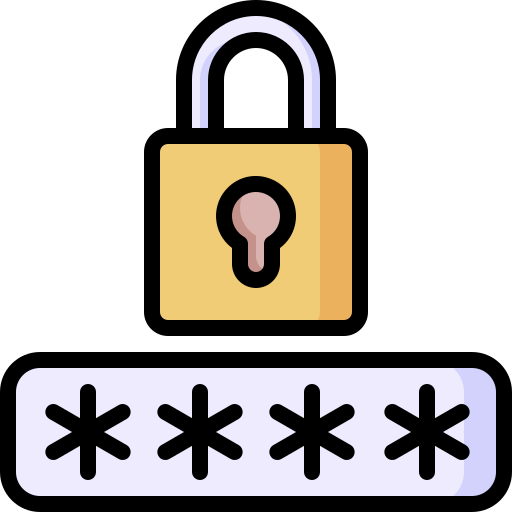
\includegraphics[height=2.5cm]{img/cadenas.png}
\end{figure}
\end{frame}

\begin{frame}
\frametitle{Fonctionnalités}
\framesubtitle {Stockage des mots de passe}
\begin{figure}[H]
\centering
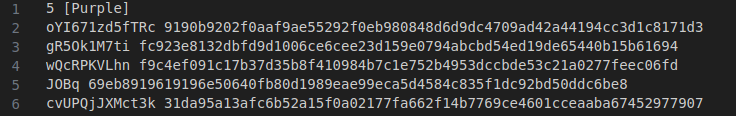
\includegraphics[height=1.8cm]{img/mdp.png}
\caption{Données dans le fichier texte}
\end{figure}
\begin{itemize}
    \item Profondeur : nombre d'itérations du processus de compression.
    \item Couleur(s) : fonction de réduction.
\end{itemize}
\end{frame}

\begin{frame}
\frametitle{Fonctionnalités}
\framesubtitle {Récupération des données}
\begin{block}{}
$\Rightarrow$ BufferedReader pour lire le fichier texte ligne par ligne.\newline
$\Rightarrow$ Première ligne extraite pour obtenir la profondeur et les couleurs.\newline
$\Rightarrow$ Les lignes suivantes sont parcourues.
\end{block}
\end{frame}

\begin{frame}
\frametitle{Fonctionnalités}
\framesubtitle {Comparaison des mots de passe}
\begin{block}{}
$\Rightarrow$ Fonctions de réduction pour obtenir le mot de passe.\newline
$\Rightarrow$ Si aucune correspondance :
\begin{itemize}
    \item  Génération de nouveaux hash à partir du hash fourni 
    \item Trouver une correspondance ou atteindre la profondeur maximale
\end{itemize}
\end{block}
\end{frame}

\begin{frame}
\frametitle{Fonctionnalités}
\framesubtitle {Fonction de réduction}
\begin{figure}[H]
    \centering
    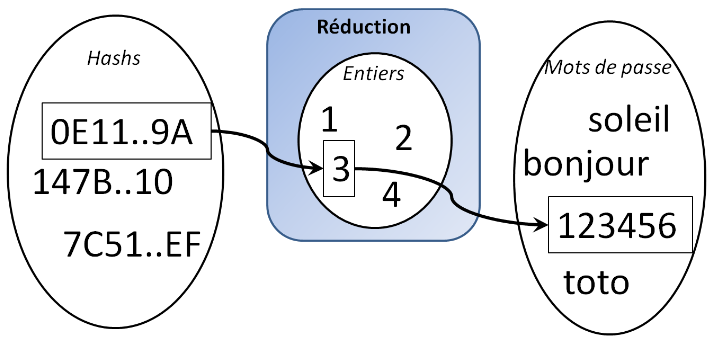
\includegraphics[height=5cm]{img/fonction_reduction.png}
    \caption{Décomposition d’une fonction de réduction}
    \end{figure}
\end{frame}

\begin{frame}
\frametitle{Fonctionnalités}
\framesubtitle {Interface graphique}
\begin{figure}[H]
\centering
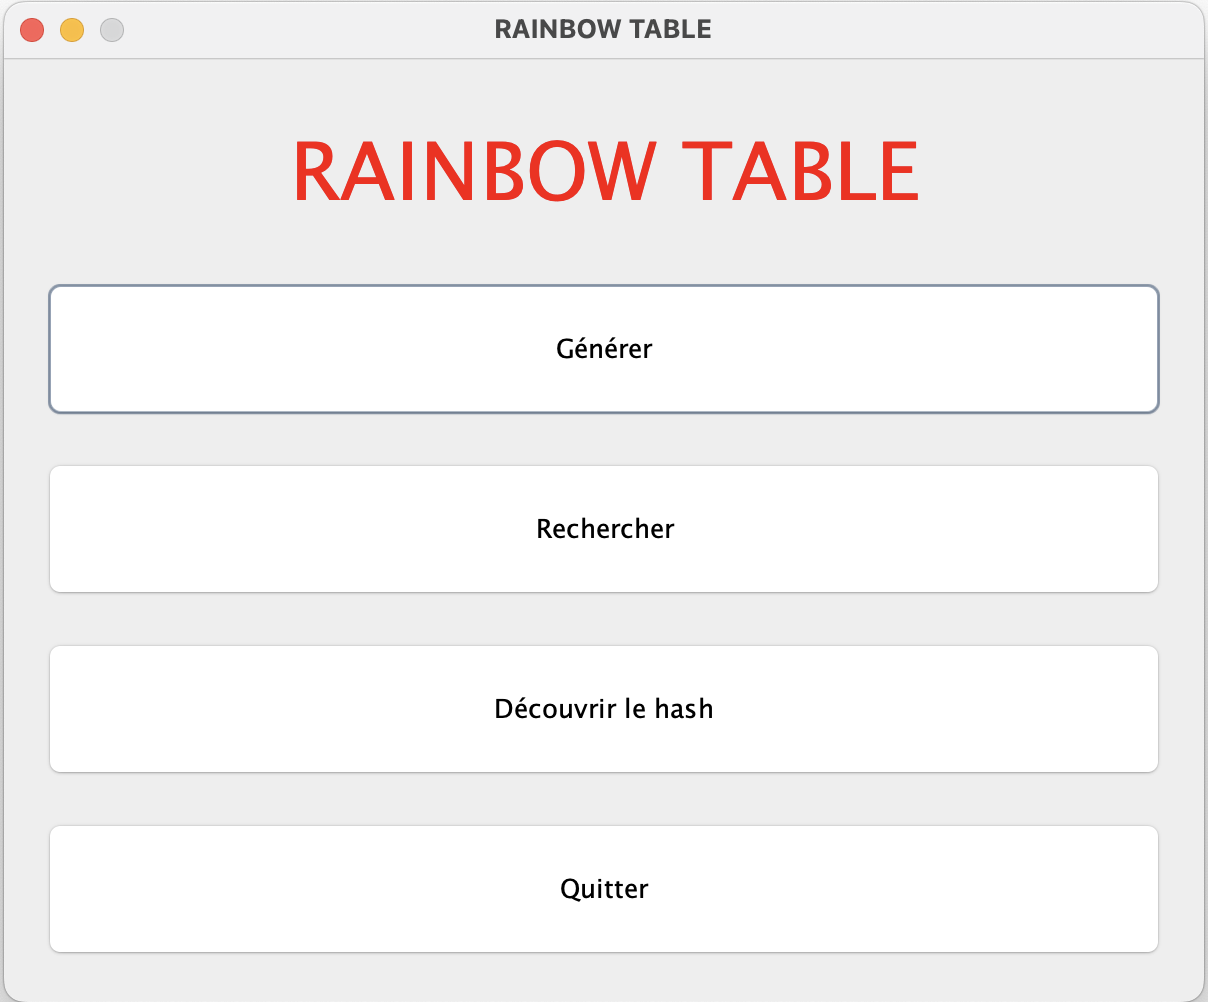
\includegraphics[height=6cm]{img/interface.png}
\caption{Interface graphique}
\end{figure}
\vfill
  \tiny *Cette capture d'écran provient de la version mac\hfill
\end{frame}

\begin{frame}
\frametitle{Fonctionnalités}
\framesubtitle {Découvrir le hash}

\begin{figure}
\centering
\begin{minipage}{0.49\textwidth}
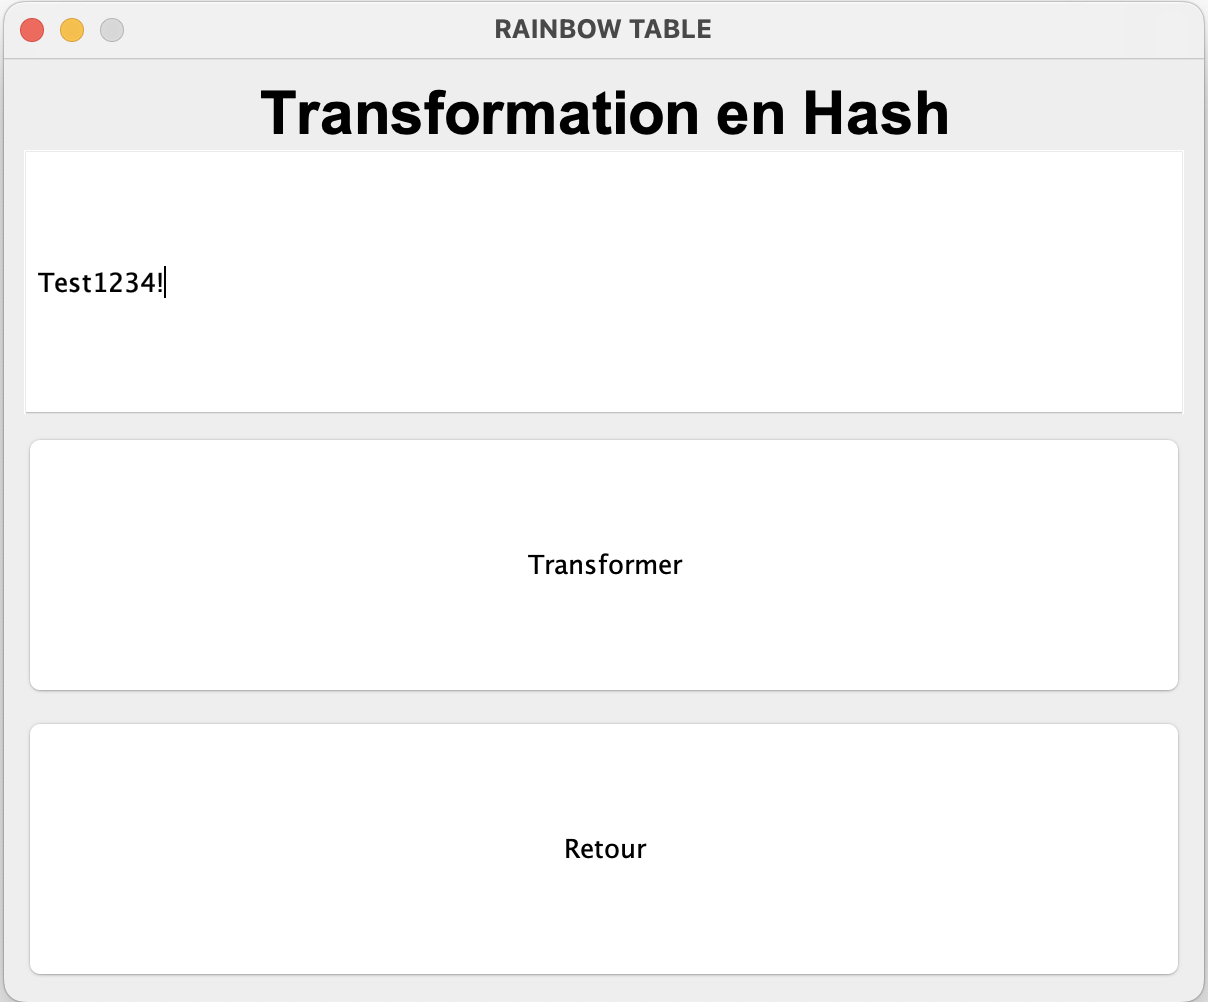
\includegraphics[height=4.8cm]{img/transform.png}
\caption{\small Mot de passe}
\end{minipage}
\begin{minipage}{0.49\textwidth}
\centering
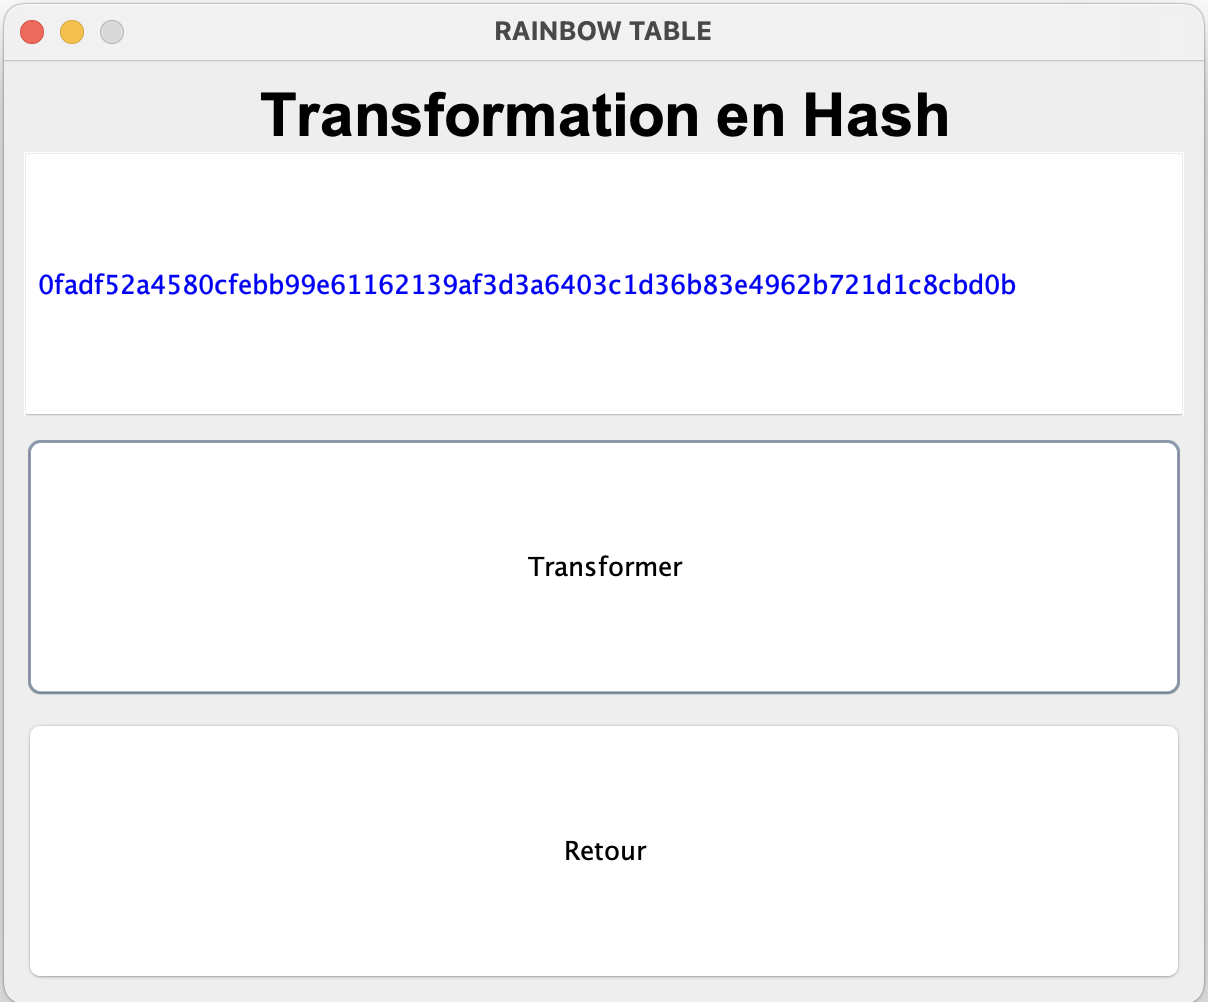
\includegraphics[height=4.8cm]{img/transform2.png}
\caption{\small Hash du mot de passe}
\end{minipage}
\end{figure}
\vfill
  \tiny *Ces captures d'écran proviennent de la version mac
\hfill
\end{frame}

\begin{frame}
\frametitle{Fonctionnalités}
\framesubtitle {Découvrir le hash}
\centering \huge Pourquoi ces choix ?
\begin{block}{}
\large
$\Rightarrow$ Plus de lisibilité : 
\begin{itemize}
    \item Hash plus reconnaissable
    \item Meilleure compréhension des fonctionnalités de cette page
\end{itemize}
$\Rightarrow$ Plus de praticité :
\begin{itemize}
    \item  Possibilité de copier coller directement dans la cellule
    \item  Retour au menu plus rapide
\end{itemize}
\end{block}{}
\end{frame}

\begin{frame}
\frametitle{Éléments techniques}
\framesubtitle {La protection}
\begin{center}
    \huge Comment se protéger des rainbow tables ?
\end{center}
\begin{figure}[H]
\centering

\includegraphics[height=3cm]{img/bouclier.png}
\end{figure}
\end{frame}

\section{Expérimentations}
\begin{frame}
\frametitle{Expérimentations}
\framesubtitle {Résultats quantifiables}
\begin{center}
    \huge Efficacité de la table en fonction des paramètres ?
\end{center}
\begin{figure}[H]
\centering
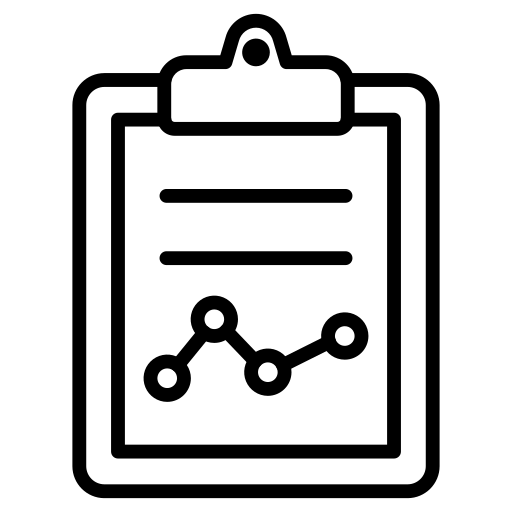
\includegraphics[height=3cm]{img/experimentation.png}
\end{figure}
\end{frame}

\begin{frame}
\frametitle{Expérimentations}
\framesubtitle {Résultats quantifiables}
\begin{figure}[H]
\centering
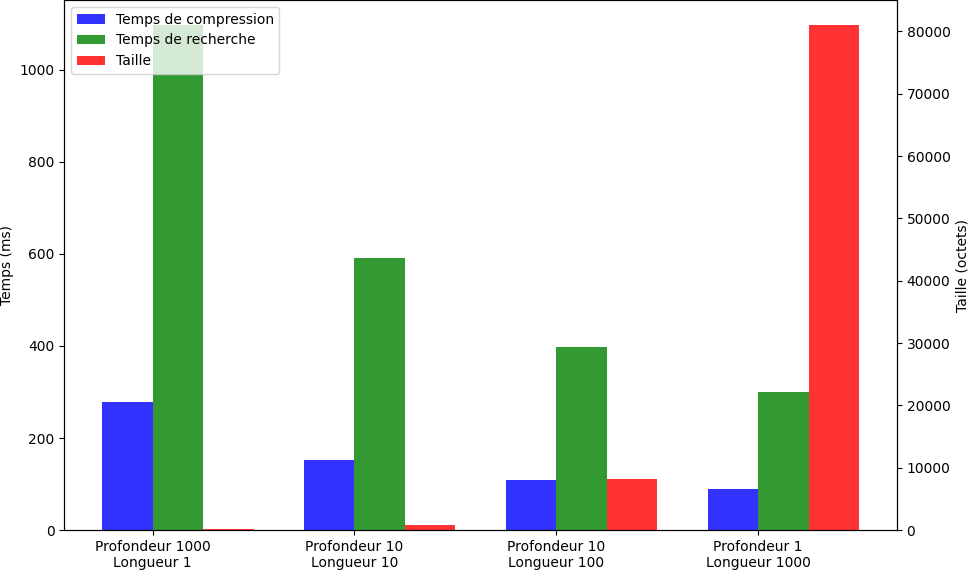
\includegraphics[height=5.5cm]{img/graphique.png}
\caption{Graphique représentant le temps de compression, de recherche et la taille en fonction de la profondeur et de la longueur}
\end{figure}
\end{frame}

\section{Conclusion}
\begin{frame}
\frametitle{Conclusion}
\framesubtitle {Avantages et inconvénients}
Avantages :
\begin{itemize}
    \item Rapidité de recherche.
\end{itemize}
Inconvénients :
\begin{itemize}
    \item Taille de stockage importante.
    \item Utilisation limitée pour les mots de passe forts.
    \item Besoin de mises à jour constantes.
\end{itemize}
\end{frame}

\begin{frame}
\frametitle{Conclusion}
\framesubtitle{Propositions d’améliorations}
\begin{columns}
\begin{column}{0.6\textwidth}
\begin{itemize}
    \item Nouveaux tests unitaires.
    \item Implémenter des optimisations connues.
    \item Système de log.
    \item Nouveaux algorithmes de hachage.
    \item Des statistiques sur l'interface.
\end{itemize}
\end{column}
\begin{column}{0.4\textwidth}
\begin{figure}[H]
\centering

\includegraphics[height=2.7cm]{img/ampoule.png}
\end{figure}
\end{column}
\end{columns}
\end{frame}

\end{document}